\documentclass[12pt,oneside]{book}

\usepackage[dvips,letterpaper,margin=0.75in,bottom=0.5in]{geometry}
\usepackage{cite}
\usepackage{slashed}
\usepackage{graphicx}
\usepackage{amsmath}
\usepackage{braket}
\begin{document}

\title{The Fourier Theorem and Applications to Physics}
\author{Michael Mulhearn}

\maketitle

\chapter{The Fourier Series}
\section{The Vector Analogy}

A vector in ordinary space is completely specified by its displacement in each spatial direction.  Lets look at this familiar picture a bit formally, to prepare us to apply it in a less intuitive (but mathematically equivalent) setting.  The first thing we will need to know how to do is to calculate the dot product between any two vectors:  
\begin{displaymath}
\vec{v} \cdot \vec{w} = v_x w_x + v_y w_y + v_z w_z 
\end{displaymath}
You already know how to do this for ordinary vectors.  In other settings, we use the more general term {\em inner product}.  To describe any vector we need a set of {\em basis vectors}, in this case $\hat{x}$, $\hat{y}$, and $\hat{z}$.  These basis vectors are orthogonal:
\begin{displaymath}
\hat{x} \cdot \hat{y} = \hat{y} \cdot \hat{z} = \hat{z} \cdot \hat{x} = 0
\end{displaymath}
and normalized:
\begin{displaymath}
\hat{x} \cdot \hat{x} = \hat{y} \cdot \hat{y} = \hat{z} \cdot \hat{z} = 1.
\end{displaymath}
When the basis vectors have both of these properties, we call them {\em orthonormal}.

For any possible vector $\vec{v}$, we can calculate its component in the direction of each basis vector by calculating the inner product of the two:
\begin{eqnarray*}
v_x = \vec{v} \cdot \hat{x} \\
v_y = \vec{v} \cdot \hat{y} \\
v_z = \vec{v} \cdot \hat{z} \\
\end{eqnarray*}
We say that the basis vectors $\hat{x}$, $\hat{y}$, and $\hat{z}$ are {\em complete}, because specifying the values of $v_x$, $v_y$, and $v_z$ completely describes the vector $\vec{v}$.  The set of basis vectors $\hat{x}$ and $\hat{z}$ are orthonormal, but they are not complete in three dimensional space, because there are vectors which we cannot write using only these two directions.  For instance, there are no possible values for $v_x$ and $v_z$
which make
\begin{eqnarray*}
 \vec{v_1} = v_x \hat{x} + v_z \hat{z}
\end{eqnarray*}
equal to the vector
\begin{eqnarray*}
 \vec{v_2} = 3 \hat{x} + 2 \hat{y} + 7 \hat{z}.
\end{eqnarray*}

 
\section{The Fourier Series in the Vector Analogy}

Using the language of vectors, the sines and cosines form a complete orthonormal basis for describing any periodic function.  To make sense of this claim, we need to define the inner product. If we restrict ourselves to real functions of $x$ with period $L$, the inner product between any two functions $f(x)$ and $g(x)$ is defined to be the integral:
\begin{equation*}
\braket{f, g} \equiv \int_{-\frac{L}{2}}^{\frac{L}{2}} f(x) g(x) \, dx
\end{equation*}
Notice that the comma between $f$ and $g$ which indicates that this is an inner product, not to be confused with an expectation value.  The orthonormal basis vectors are the specific sine and cosine functions
\begin{eqnarray*}
s_n(x) \equiv \sqrt{\frac{2}{L}}\sin\left(\frac{2\pi n}{L} \, x \right)\\
c_n(x) \equiv \sqrt{\frac{2}{L}}\cos\left(\frac{2\pi n}{L} \, x \right)
\end{eqnarray*}
which are defined for $n=1,2,3,\ldots$.  They are normalized because by our definition for the inner product we can see that:
\begin{eqnarray*}
\braket{s_n, s_n} &=& \frac{2}{L} \int_{-\frac{L}{2}}^{\frac{L}{2}} \sin^2\left(\frac{2\pi n}{L} \, x \right) \, dx = 1 \\
\braket{c_n, c_n} &=& \frac{2}{L} \int_{-\frac{L}{2}}^{\frac{L}{2}} \cos^2\left(\frac{2\pi n}{L} \, x \right) \, dx = 1
\end{eqnarray*}
The demonstration that they are orthogonal:
\begin{eqnarray}
\braket{s_n, s_m} &=& \frac{2}{L} \int_{-\frac{L}{2}}^{\frac{L}{2}} 
\sin\left(\frac{2\pi n}{L} \, x \right) \sin\left(\frac{2\pi m}{L} \, x \right) \, dx = 0 ~~(n \neq m) \label{eqn:trigortha} \\
\braket{c_n, c_m} &=& \frac{2}{L} \int_{-\frac{L}{2}}^{\frac{L}{2}} 
\cos\left(\frac{2\pi n}{L} \, x \right) \cos\left(\frac{2\pi m}{L} \, x \right) \, dx = 0~~(n \neq m) \label{eqn:trigorthb}\\
\braket{s_n, c_m} &=& \frac{2}{L} \int_{-\frac{L}{2}}^{\frac{L}{2}} 
\sin\left(\frac{2\pi n}{L} \, x \right) \cos\left(\frac{2\pi m}{L} \, x \right) \, dx = 0 \label{eqn:trigorthc}
\end{eqnarray}
which follows from the identities:
\begin{eqnarray*}
\sin \alpha \sin \beta &=& \frac{1}{2} \{\cos(\alpha - \beta) - \cos(\alpha + \beta)\}\\
\cos \alpha \cos \beta &=& \frac{1}{2} \{\cos(\alpha - \beta) + \cos(\alpha + \beta)\}\\
\cos \alpha \sin \beta &=& \frac{1}{2} \{\sin(\alpha + \beta) - \sin(\alpha - \beta)\}\\
\end{eqnarray*}
is left as an exercise.

We combine the normalization and orthogonality conditions using the Kronecker delta symbol:
\begin{displaymath}
\delta_{nm} =  
\left\{
	\begin{array}{ll}
		1  & \mbox{if } n=m \\
		0 & \mbox{otherwise}
	\end{array}
\right.
\end{displaymath}
and write the above five equations compactly as:
\begin{eqnarray}
\braket{s_n, s_m} &=&  \delta_{nm} \nonumber \\
\braket{c_n, c_m} &=&  \delta_{nm} \label{eqn:coscos} \\
\braket{s_n, c_m} &=&  = 0 \nonumber
\end{eqnarray}

The sines and functions are {\em complete}, which means that any periodic function with period $L$ can be written as an infinite sum of sines and cosines plus a constant value $C$:
\begin{eqnarray}
f(x) = \sqrt{\frac{2}{L}} \sum_{n=1}^{\infty}  A_n \, \cos\left(\frac{2\pi n}{L} \, x \right) + \sqrt{\frac{2}{L}}  \sum_{n=1}^{\infty} B_n \, \sin\left(\frac{2\pi n}{L} \, x \right) + C\label{eqn:bigseries}
\end{eqnarray}
The values $A_n$, $B_n$,  are called {\em Fourier coefficients}.   As we will see, there are different conventions for handling the constant term $C$.  Technically the $n$th term in the Fourier Series refers to the approximation for $f(x)$ from the first $N$ terms in the infinite sum above, and we say that the Fourier Series converges to the function $f(x)$.  The demonstration of completeness of the sines and cosines is in the Appendix.  For a visual example of the Fourier Series, the first terms of the Fourier Series for a step function are shown in Fig.~\ref{fig:fall}.  

\begin{figure}[thb]
\begin{center}
{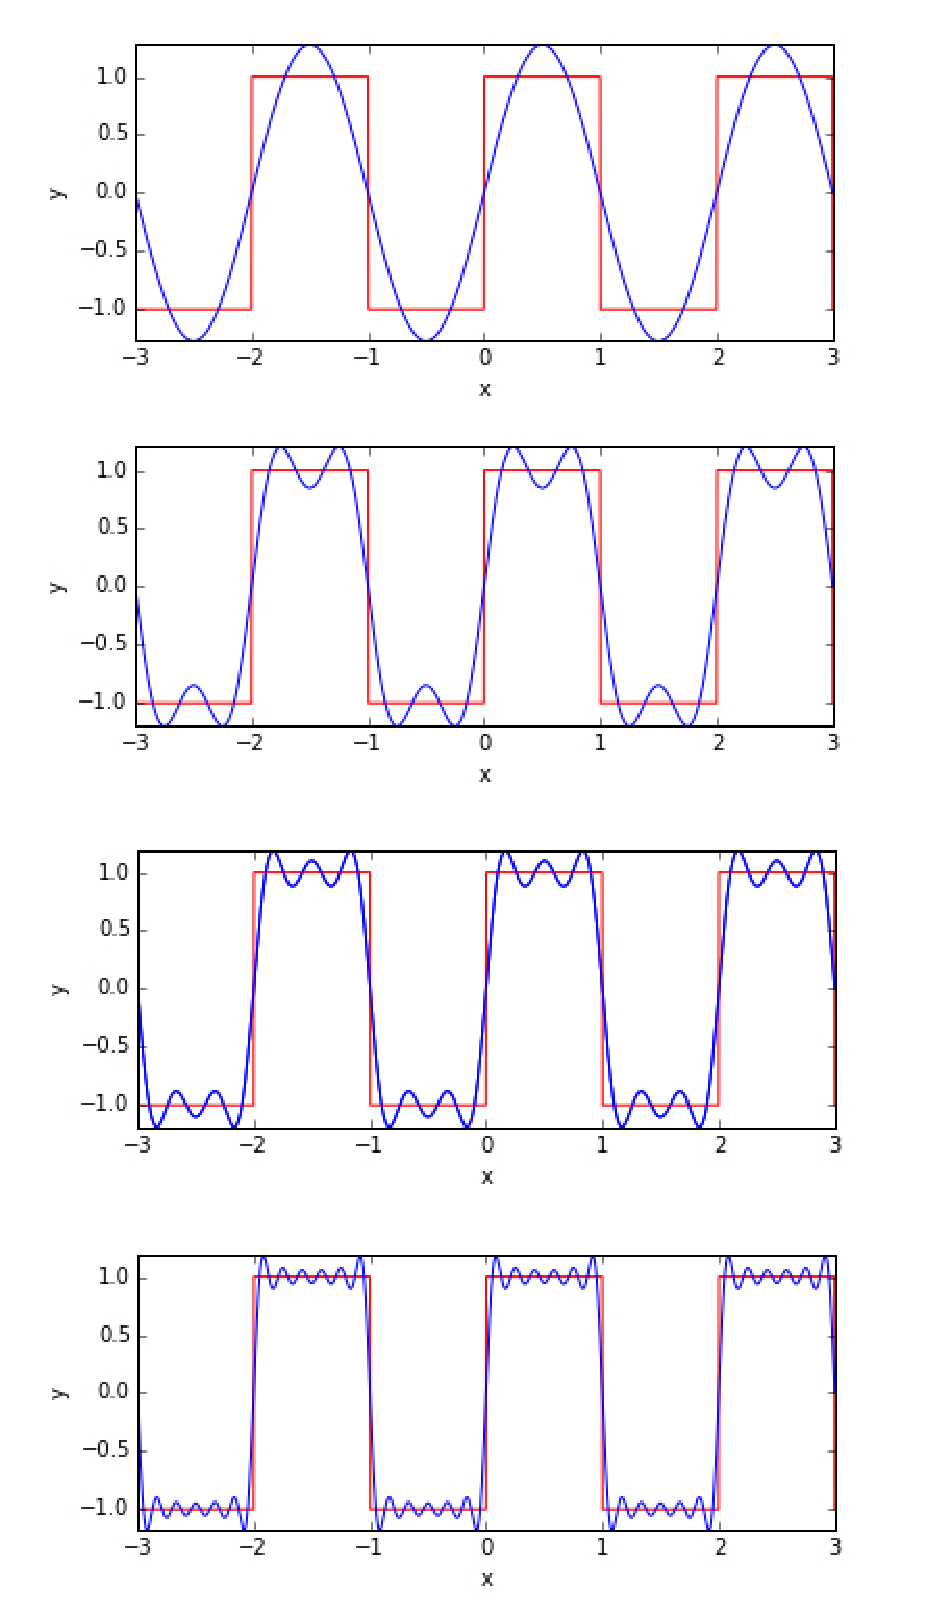
\includegraphics[width=0.35\textwidth]{figs/fsall.pdf}}
\end{center}
\caption{\label{fig:fall} The Fourier Series for a step function including one term, three terms, five terms, and nineteen terms.  The Fourier Theorem states that the series will converge, reproducing the original function, as the number of terms approaches infinity.}
\end{figure}

\section{Determining the Fourier Coefficients}
\label{sect:coeff}


Just as in the vector analogy, we can determine the Fourier coefficients of a function $f$ by computing the inner products:
\begin{eqnarray*}
A_n = \braket{c_n, f} \\
B_n = \braket{s_n, f} 
\end{eqnarray*}
or, in terms of the inner product integrals:
\begin{eqnarray}
A_n &=& \sqrt{\frac{2}{L}} \int_{-\frac{L}{2}}^{\frac{L}{2}} 
\cos\left(\frac{2\pi n}{L} \, x \right) \, f(x) \, dx \label{eqn:fca} \\
B_n &=& \sqrt{\frac{2}{L}} \int_{-\frac{L}{2}}^{\frac{L}{2}} \nonumber
\sin\left(\frac{2\pi n}{L} \, x \right) \, f(x) \, dx
\end{eqnarray}
The constant term $C$ is the average value of the function across one period:
\begin{equation*}
C = \frac{1}{L} \int_{-\frac{L}{2}}^{\frac{L}{2}} f(x) \, dx
\end{equation*}
An alternative approach is to define $c_0 = 1/\sqrt{L}$vwhich you can think of as a properly normalized $\cos(0)$ function, in which case the Fourier coefficient $A_0$ becomes the constant term.

Just as in the vector analogy, the inner product determines the correct coefficients only because the basis functions are complete and orthonormal.  For convenience, we will demonstrate this with a function that has $C$ and all of the $B_n$ coefficients equal to zero.  Start with the completeness equation, but change the index from $n$ to $m$ in order to make the next step clearer.  
\begin{displaymath}
f(x) = \sqrt{\frac{2}{L}} \sum_{m=1}^{\infty}  A_m \, \cos\left(\frac{2\pi m}{L} \, x \right)
\end{displaymath}
Now we apply the prescription in Equation~\ref{eqn:fca} to both sides of this equation:
\begin{eqnarray*}
\sqrt{\frac{2}{L}} \int_{-\frac{L}{2}}^{\frac{L}{2}} 
\cos\left(\frac{2\pi n}{L} \, x \right) \, f(x) \, dx  
&=& \sqrt{\frac{2}{L}} \int_{-\frac{L}{2}}^{\frac{L}{2}} 
\cos\left(\frac{2\pi n}{L} \, x \right) \,
\left\{
\sqrt{\frac{2}{L}} \sum_{m=0}^{\infty}  A_m \, \cos\left(\frac{2\pi m}{L} \, x \right) \right\}
 \, dx \\
&=& \sum_{m=0}^{\infty}  A_m \, \left\{ \frac{2}{L} 
\int_{-\frac{L}{2}}^{\frac{L}{2}} 
 \, \cos\left(\frac{2\pi n}{L} \, x \right) \cos\left(\frac{2\pi m}{L} \, x \right) \, dx \right\}\\
&=& \sum_{m=0}^{\infty}  A_m \, \delta_{nm} \\
&=& A_n
\end{eqnarray*}

\section{Compact Form of the Fourier Series}

The Fourier Series developed above has the considerable advantage that it makes explicit the role of the sine and cosine functions as an orthonormal basis.  But it is a bit unwieldy and seldom encountered in that form for practical applications.  Consider Equation~\ref{eqn:bigseries} again:
\begin{eqnarray*}
f(x) = \sqrt{\frac{2}{L}} \sum_{n=0}^{\infty}  A_n \, \cos\left(\frac{2\pi n}{L} \, x \right) + \sqrt{\frac{2}{L}} \sum_{n=1}^{\infty} B_n \, \sin\left(\frac{2\pi n}{L} \, x \right) + C
\end{eqnarray*}
It is convenient to absorb the normalization factor $\sqrt{2/L}$ into the coefficients.  The series is therefore most often written in the much more compact form:
\begin{eqnarray}
f(x) = \frac{a_0}{2} + \sum_{n=1}^{\infty}  \left\{ a_n \, \cos(k_n x ) + b_n \, \sin( k_n x ) \right\}\label{eqn:convseries}
\end{eqnarray}
where we have also introduced the wave numbers:
\begin{equation}
k_n \equiv \frac{2 \pi n}{L} \label{eqn:kn}
\end{equation}
and the new Fourier Coefficients:
\begin{eqnarray}
a_n &\equiv& \sqrt{\frac{2}{L}}  A_n = \frac{2}{L} \int_{-\frac{L}{2}}^{\frac{L}{2}} 
f(x) \cos( k_n x) \, dx  \label{eqn:convcoeffa}\\
b_n &\equiv& \sqrt{\frac{2}{L}}  B_n = \frac{2}{L} \int_{-\frac{L}{2}}^{\frac{L}{2}} 
f(x) \sin( k_n x) \, dx \label{eqn:convcoeffb}
\end{eqnarray}
Notice that this definition correctly determines the coefficient $a_0$ for the constant factor because $\cos(0) = 1$.

\section{Fourier Series for Complex Functions}

The Fourier Series can be expressed in terms of the complex exponential by noting that:
\begin{eqnarray*}
\cos(k_n x) &=& \frac{\exp(i k_n x) + \exp(-i k_n x)}{2} \\
\sin(k_n x) &=& \frac{\exp.(i k_n x) - \exp(-i k_n x)}{2i}
\end{eqnarray*}
So that Equation~\ref{eqn:convseries} can be rewritten as:
\begin{eqnarray}
f(x) &=& \frac{a_0}{2} + \sum_{n=1}^{\infty}  \left\{ a_n \, \cos(k_n x ) + b_n \, \sin( k_n x ) \right\} \nonumber \\
&=& \frac{a_0}{2}+ \sum_{n=1}^{\infty}  \left\{ a_n \,  \frac{\exp(i k_n x) + \exp(-i k_n x)}{2} 
+ b_n \, \frac{\exp(i k_n x) - \exp(-i k_n x)}{2i} \right\} \nonumber \\
&=& \frac{a_0}{2} + \sum_{n=1}^{\infty}  \left\{ \frac{a_n - i b_n}{2} \exp(i k_n x) + 
\frac{a_n + i b_n}{2} \exp(-i k_n x) \right\} \nonumber \\
&=& c_0 + \sum_{n=1}^{\infty}  \left\{ c_n \exp(i k_n x) + 
c_n^* \exp(-i k_n x) \right\}  \label{eqn:bigcomplex}
\end{eqnarray}
Where in the last step we have introduced the complex Fourier coefficient:
\begin{equation}
c_n \equiv \frac{a_n - i b_n}{2}. \label{eqn:defcomplex}
\end{equation}
Notice in Equation~\ref{eqn:bigcomplex} that $c_0$ is real because $b_0 = 0$ in Equation~\ref{eqn:defcomplex}, and each summand in the sum is of the form $z+z^*$, hence $f(x)$ is real, as we assumed initially.  Each summand in Equation~\ref{eqn:bigcomplex} is of form $z+z^*$ because the coefficients of the complex exponentials are complex conjugates.  If we replace our initial real function $f(x) $ with a complex valued function $\Psi(x)$ (such as a wave function in Quantum Mechanics!), the constraint that these coefficients are complex conjugates vanishes, and we can replace $c_n^*$ with new independent\footnote{If you prefer, you can construct the complex function from two real functions:  $\Psi(x) = f(x) + i g(x)$.  Either way, you have twice as many independent Fourier coefficients when the function is complex valued.} complex Fourier coefficients $d_n$.   Furthermore, the constant $c_0$ which was real is now allowed to be complex.
\begin{eqnarray*}
\Psi(x)  &=& c_0 + \sum_{n=1}^{\infty}  \left\{ c_n \exp(i k_n x) + 
d_n \exp(-i k_n x) \right\} 
\end{eqnarray*}
And finally, we note that we can simplify this equation even further by being quite clever, noting that 
$k_{(-n)} = -k_n$ and defining $c_{(-n)} \equiv d_n$:
\begin{eqnarray}
\Psi(x)  &=& c_0 + \sum_{n=1}^{\infty}  c_n \exp(i k_n x) + \sum_{n=1}^{\infty}  d_n \exp(-i k_n x) \nonumber \\
 &=& c_0 + \sum_{n=1}^{\infty}  c_n \exp(i k_n x) + \sum_{n=-\infty}^{-1}  c_n \exp(i k_n x) \nonumber \\
\Psi(x) &=& \sum_{n=-\infty}^{\infty} c_n \exp(i k_n x). \label{eqn:complexseries}
\end{eqnarray}
Its amusing to compare the size of Equation~\ref{eqn:bigseries} with Equation~\ref{eqn:complexseries}, and note that the latter form is considerably more powerful.  To determine the complex Fourier coefficients we calculate:
\begin{eqnarray}
c_n &\equiv& \frac{a_n - i b_n}{2}. \nonumber \\
&=& \frac{1}{2} \left\{ 
\frac{2}{L} \int_{-\frac{L}{2}}^{\frac{L}{2}}  \Psi(x) \cos( k_n x) \, dx
-i \frac{2}{L} \int_{-\frac{L}{2}}^{\frac{L}{2}}  \Psi(x) \sin( k_n x) \, dx
\right\} \nonumber \\
&=& \frac{1}{L} \int_{-\frac{L}{2}}^{\frac{L}{2}}  \Psi(x) \left\{\cos( k_n x) - i \sin( k_n x) \right\} \, dx \nonumber \\
c_n &=& \frac{1}{L} \int_{-\frac{L}{2}}^{\frac{L}{2}}  \Psi(x) \exp(-i k_n x) \, dx \label{eqn:complexcoeff}
\end{eqnarray}

Now look closely at Equation~\ref{eqn:complexseries} and Equation~\ref{eqn:complexcoeff} and spot the negative sign in the exponential function of the latter.  It seems something strange has happened.  Instead of the sines and cosines, we would like to think of our new orthonormal basis as the complex exponential functions 
\begin{equation}
e_n(x) \equiv \frac{1}{\sqrt{L}}\exp(i k_n x).  
\end{equation}
But to calculate the coefficient of $\exp(i k_n x)$, we integrate with respect to a {\em different} function $\exp(-i k_n x)$.  Can our vector analogy survive this?  It seems as though we are calculating the component along $\hat{x}$ by taking the dot product with $-\hat{x}$.   

It turns out that for complex valued functions, we need to modify our inner product to include complex conjugation of one of the functions:
\begin{equation}
\braket{\Psi, \phi} \equiv \int_{-\frac{L}{2}}^{\frac{L}{2}} \Psi^*(x) \phi(x) \, dx
\end{equation}
With this simple tune up, the vector analogy for complex valued functions is saved!   We still have orthonormal basis functions:
\begin{eqnarray}
\braket{e_n, e_m} &=& \frac{1}{L} \int_{-\frac{L}{2}}^{\frac{L}{2}}  \exp(-i k_n x) \exp(k_m x) \, dx \nonumber \\
&=& \delta_{nm} \label{eqn:exportho}
\end{eqnarray}
and we still calculate the coefficient of each $e_n(x)$ from the inner product:
\begin{equation}
c_n = \braket{e_n, \Psi} = \frac{1}{L} \int_{-\frac{L}{2}}^{\frac{L}{2}}  \Psi(x) \, \exp(-i k_n x) \; dx
\end{equation}

\chapter{The Fourier Transform}

\section{Non-periodic Functions}
The Fourier Series is sufficient for periodic functions.  In this chapter, we will extend the Fourier series concept to apply to any function, with the only caveat that the function must approach zero as $x$ approaches both negative and positive infinity.  The trick is to consider such a function as periodic with period $L$ in the limit $L \to \infty$.  Recall Equation~\ref{eqn:kn}:
\begin{equation*}
k_n \equiv \frac{2 \pi n}{L}.
\end{equation*}
When $L$ is very large, we will obtain a non-zero value for $k_n$ only for comparably large values of $n$.  But since $n$ is very large, the difference between $k_n$ and $k_{n+1}$ is infinitesimal.  We have moved from the discreet case, where we only have certain wave numbers $k_n$ for each integer $n=0,1,2,...$, to the continuous case, where $k$ can take any real value.  Fortunately, our vector analogy survives intact!

Our inner product now extends between positive and negative infinity:
\begin{equation}
\braket{\Psi, \phi} \equiv \int_{-\infty}^{\infty} \Psi^*(x) \phi(x) \, dx
\end{equation}
Our basis functions, which are now defined for any value of $k$,
\begin{equation}
e_k = \frac{1}{\sqrt{2\pi}} \exp(i k x)
\end{equation}
are still orthonormal, but the condition looks a bit different in the continuum case:
\begin{eqnarray*}
\braket{e_k, e_{k'}} &=& \delta(k-k')
\end{eqnarray*}
See the appendix for more details on the Dirac delta function $\delta(x)$, which is zero everywhere but at $x=0$, where it is infinite.  It is the continuous version of $\delta_{nm}$.

Our basis functions are also still complete.  In the discrete case we have a complex Fourier coefficient for every integer $n$.   Now we have a complex Fourier coefficient for any real value of $k$.  In place of Fourier coefficients, we have instead a function of $k$ which we call the Fourier transform: $\widetilde{\Psi}(k)$.
Instead of a sum over discrete terms, we now have to integrate over all values of $k$:
\begin{equation} \label{eqn:ift}
\Psi(x) = \frac{1}{\sqrt{2\pi}} \int_{-\infty}^{\infty} \widetilde{\Psi}(k) \exp(ikx) \, dk.
\end{equation}
Just as in the discrete case, we determine the Fourier transform from the inner product:
\begin{equation} \label{eqn:ft}
\widetilde{\Psi}(k) = \braket{e_k, \Psi} = \frac{1}{\sqrt{2\pi}} \int_{-\infty}^{\infty} {\Psi}(x) \exp(-ikx) \, dx
\end{equation}
Equation~\ref{eqn:ft} is generally referred to as the {\em Fourier Transform}, while Equation~\ref{eqn:ift} is referred to as the {\em Inverse Fourier Transform}.

\section{Fourier Pairs}

So far we have restricted ourselves to considering functions of a variable $x$ and wave number $k$, so that $k x$ is a dimensionless quantity suitable for evaluating a sine, cosine, or exponential function.
In fact, any dimensionless quantity composed from two variables can be the basis of a Fourier analysis.
One of the more confusing aspects of the Fourier Theorem is the bewildering variation in the applications, and different conventions.   But this is merely an inevitable consequence of how fundamental and powerful a tool it is.  

As Fourier pairs we most often see the dimensionless quantities $k\,x$, $p\,x/\hbar$, $\omega \, t$, $2\pi \, f \, t$, and $E \, t/\hbar$.  Once the Fourier pair is chosen, one then has to decide how to normalize the Fourier Transform and Inverse Fourier Transform, that is, how to absorb additional constants like $\hbar$ and $2 \pi$.  But whatever unfamiliar ground you find yourself on, it is always true that:
\begin{displaymath}
\int^{\infty}_{-\infty} \exp(ikx) \, dx = 2\pi \, \delta(k),
\end{displaymath}
which can be used to determine consistent definitions.

A popular choice for the Fourier is frequency and time.  In this case, we have simply:
\begin{eqnarray}
\widetilde{V}(f) &=& \int^{\infty}_{-\infty}\exp(-i2\pi f t) \; V(t) \, dt \\
V(t) &=& \int^{\infty}_{-\infty}\exp(i2\pi f t) \; \widetilde{V}(f) \, df \\
\end{eqnarray}

\chapter{Power Spectral Density}

\section{Energy Spectral Density}
Consider:
\begin{eqnarray*}
\int_{-\infty}^{\infty} dt \; |V(t)|^2 &=&  \int_{-\infty}^{\infty} dt \, V^*(t) \; V(t) \\
&=& \int_{-\infty}^{\infty} dt \, \left( \frac{1}{\sqrt{2\pi}} \int_{-\infty}^{\infty} df \, \widetilde{V}(f) \exp(-i2\pi f t) \right)^*  \left( \frac{1}{\sqrt{2\pi}} \int_{-\infty}^{\infty} df' \, \widetilde{V}(f') \exp(-i2\pi f' t) \right) \\
&=& \int_{-\infty}^{\infty} dt \, \left( \frac{1}{\sqrt{2\pi}} \int_{-\infty}^{\infty} df \, \widetilde{V}^*(f) \exp(i2\pi f t) \right)  \left( \frac{1}{\sqrt{2\pi}} \int_{-\infty}^{\infty} df' \, \widetilde{V}(f') \exp(-i2\pi f' t) \right) \\
&=& \int_{-\infty}^{\infty} df \int_{-\infty}^{\infty} df'  \; \widetilde{V}^*(f) \, \widetilde{V}(f') 
\; \int_{-\infty}^{\infty} dt \exp(i2\pi(f-f')t)\\
&=& \int_{-\infty}^{\infty} df \int_{-\infty}^{\infty} df'  \; \widetilde{V}^*(f) \, \widetilde{V}(f') 
\; \delta(f-f')\\
&=& \int_{-\infty}^{\infty} df \; |\widetilde{V}(f)|^2
\end{eqnarray*}
which is called Parseval's Theorem.  In all of it's guises, Parseval's Theorem relates the integrated squared-norm of a function to that of its Fourier transform.  But take care that sometimes there are additional normalization factors.   For instance, if we chose to use $\omega = 2 \pi f$ instead of $f$ as the Fourier conjugate variable, we find that:
\begin{displaymath}
\int_{-\infty}^{\infty} dt \; |V(t)|^2 = \frac{1}{2\pi}\int_{-\infty}^{\infty} d\omega \; |V(\omega)|^2
\end{displaymath}
In many cases, the power of a time varying signal goes as an amplitude squared.  For example, the energy stored in a capacitor is:
\begin{displaymath}
U = \frac{1}{2} C V^2
\end{displaymath}
and so the total energy of time dependent voltage can be calculated as:
\begin{equation}
E \propto \int |V(t)|^2 \, dt \label{eqn:energy}
\end{equation}
but Parseval's theorem implies that also:
\begin{displaymath}
E \propto \int |\widetilde{V}(f)|^2 \, df
\end{displaymath}
We can therefore associate the quantity $|\widetilde{V}(f)|^2$, which we call the Energy Spectral Density, with the amount of energy contained in the signal at frequency $f$:
\begin{displaymath}
\frac{dE }{df} \propto |\widetilde{V}(f)|^2 
\end{displaymath}

\section{Autocorrelation}

We define the autocorrelation of a function of time $V(t)$ as the integral of the function with a copy of itself delayed by time $\tau$:
\begin{equation}
R(\tau) \equiv \int^{\infty}_{-\infty} du \; V(u) \, V(u-\tau) \label{eqn:auto}
\end{equation}
Notice that $R(-\tau) = R(\tau)$ (by changing integration variables).  Also notice that $R(\tau) \leq R(0)$, that is, $R$ is monotonically decreasing.  For most (non-periodic) physical signals, the autocorrelation vanishes quickly away from the origin.  Consider the Fourier Transform $S(f)$ of the autocorrelation function when the Fourier transforms of the signal $V$ can be calculated:
\begin{eqnarray*}
S(f) &\equiv&  \int_{-\infty}^{+\infty} d\tau \, R(\tau) \exp(-i2\pi \tau) \\
&=& \int_{-\infty}^{+\infty} du \, \int_{-\infty}^{+\infty} d\tau \, V(u) \, V(u-\tau) \, \exp(-i2\pi \tau) \\
&=& \int_{-\infty}^{+\infty} du \; V(u) \, \exp(i2\pi u) \, \left\{ \int_{-\infty}^{+\infty} d\tau \, V(u-\tau) \, \exp(-i2\pi(u-\tau)) \right\}\\
&=& \int_{-\infty}^{+\infty} du \; V(u) \, \exp(i2\pi \tau) \left\{ \int_{-\infty}^{+\infty} dv \, V(v) \, \exp(-i2\pi v) \right\}\\
&=& | \widetilde{V}(f) |^2 \propto \frac{dE}{df}
\end{eqnarray*}
So the Fourier Transform of the Autocorrelation function is the Energy spectral density.  This fascinating outcome is quite useful in physics, as we shall see.  As the Fourier transform measures the amplitude of the periodic functions contained within a signal, and the autocorrelation function preserves the periodicity of the original function, it makes sense intuitive sense that the autocorrelation function still contains the information needed to determine the energy spectral density.

\section{Power Spectral Density}

The definitions above work well for a limited time duration pulses with finite total energy, when the integral in Equation~\ref{eqn:energy} is calculable.  However, for continuous signals, that are present for all time, the total energy is infinite and so the energy spectral density is undefined.  Yet it certainly makes sense to ask what the frequency distribution of a continuous signal is.  The answer is to normalize these distribution, essentially turning them into expectation values with respect to time.  Even if this integral diverges:
\begin{displaymath}
\int_{-\infty}^{\infty} dt \; f(t) \to \infty
\end{displaymath}
this limit, because of the normalization factor $T$, will often converge:
\begin{displaymath}
\lim_{T \to \infty } \frac{1}{T} \int_{-T/2}^{T/2} f(t) \, dt \; \equiv \braket{f(t)},
\end{displaymath}
and represents the expectation value of $f$ over all time.  For $f(t) = V^2(t)$ the integral in Equation~\ref{eqn:energy} yielded the total energy, while this expectation value gives the average power: 
\begin{equation}
P_{\rm avg} \propto \lim_{T\to \infty} \frac{1}{T} \int_{-T/2}^{T/2} dt \, |V(t)|^2 \label{eqn:power} = \braket{V^2(t)} = V^2_{\rm RMS}
\end{equation}
Signals with a finite energy are called ``energy signals'' and have a well-defined energy spectral density.
Signals with a finite average power and therefore infinite energy are called ``power signals''.  Of course, there are no actual power signals in the universe, but many signals last much longer than the time interval of interest, and are therefore effectively power signals.

When it exists, the Fourier transform $\widetilde{V}(f)$ contains useful information about the frequency distribution of a power signal.  However, there are many important cases, such as for random noise, that the Fourier transform of $V(t)$ does not exist.  Recall that for energy signals, the Fourier transform of the autocorrelation gave the energy spectral density.  In this case, the correlation function as defined in Equation~\ref{eqn:auto} diverges, but if we normalize it:
\begin{equation}
\mathcal{R}(\tau) \equiv \lim_{T \to \infty } \frac{1}{T} \int_{-T/2}^{T/2} dt \; V(t) \, V(t-\tau) = \braket{V(t) \, V(t-\tau)}
\label{eqn:autopower}
\end{equation}
this function is usually well behaved, and part of a Fourier Transform pair:
\begin{eqnarray}
\mathcal{S}(f) &\equiv& \int_{\infty}^{-\infty} d\tau \; \mathcal{R}(\tau) \exp(-i2\pi f \tau) \\ 
\mathcal{R}(\tau) &=& \int_{\infty}^{-\infty} df \; \mathcal{S}(f) \exp(i2\pi f \tau)  \label{eqn:ifts}
\end{eqnarray}
But how should we interpret $\mathcal{S}(f)$ which we hope contains useful information about the frequency distribution of our signal?  We start by noting that Definition~\ref{eqn:autopower} implies
that:
\begin{displaymath}
\mathcal{R}(0) = \braket{V^2(t)} = V^2_{\rm RMS} \propto P_{\rm avg}
\end{displaymath}
but from Equation~\ref{eqn:ifts} we also have:
\begin{eqnarray*}
\mathcal{R}(0) &=& \int_{\infty}^{-\infty} df \; \mathcal{S}(f) \exp(i2\pi f 0) \\
        &=& \int_{\infty}^{-\infty} df \; \mathcal{S}(f)
\end{eqnarray*}
or in other words:
\begin{displaymath}
P_{\rm avg} \propto  \braket{V^2(t)} = \int_{\infty}^{-\infty} df \; \mathcal{S}(f) 
\end{displaymath}
That is to say $\mathcal{S}(f)$ is the average power contained at frequency $f$:
\begin{displaymath}
\mathcal{S}(f) \propto \frac{dP_{\rm avg}}{df}
\end{displaymath}
 To calculate $\mathcal{S}(f)$ we simply calculate the Fourier transform of the autocorrection function:
\begin{equation}
\mathcal{R}(\tau) \equiv \braket{V(t) V(t-\tau)}.
\end{equation}

There are a few practical simplifications we can make resulting from the fact that $\mathcal{R}(\tau)$
is a real even function, and therefore need only calculate:
\begin{displaymath}
\mathcal{S}(f) =2  \int^{\infty}_{0} d\tau \; \mathcal{R}(\tau) \cos(2\pi f \tau).
\end{displaymath}
But now clearly $\mathcal{S}(f)$ is also an even function, and we can therefore consider the one-sided-power spectral distribution:
\begin{eqnarray}
\mathcal{S}_{+}(f) &\equiv& 2 \, \mathcal{S}(f) \\ 
&=& 4  \int^{\infty}_{0} d\tau \; \mathcal{R}(\tau) \cos(2\pi f \tau) 
\end{eqnarray}
which has the same interpretation as the power spectral distribution but simply restricted to positive frequencies:
\begin{equation}
P_{\rm avg} \propto \braket{V^2(t)} = \int_{0}^{\infty} df \; \mathcal{S}_+(f) 
\end{equation}

\section{The Periodogram}

Consider the Fourier series for a period function of time with period $T$:
\begin{displaymath}
V(t) = \sum_n c_n \exp(i 2 \pi f_n \, t)
\end{displaymath}
where $f_n = n / T$ are the discrete frequencies of the series.
To reproduce Parseval's Theorem in this context, we calculate:
\begin{eqnarray*}
\int_{-T/2}^{T/2} dt \; |V(t)|^2 &=&  \int_{-T/2}^{T/2} df \, V^*(t) \; V(t) \\
&=& \int_{-\infty}^{\infty} df \, \left( \sum_m c_m \exp(i 2 \pi f_m \, t) \right)^*  \left( \sum_n c_n \exp(i 2 \pi f_n \, t) \right) \\
&=& \sum_m \; \sum_n c_m^* c_n \int_{-T/2}^{T/2} df \, \exp(- i 2 \pi f_m t) \, \exp(i 2 \pi f_n t) \\
&=& \sum_m \; \sum_n c_m^* c_n \, T \, \delta_{nm} \\
&=& T \, \sum_n \, |c_n|^2 \\
\end{eqnarray*}
where we have picked up a factor of the period $T$, so that Parseval's Theorem is better written in this context as:
\begin{displaymath}
\frac{1}{T} \int_{-T/2}^{T/2} dt \; |V(t)|^2 = \sum_n \, |c_n|^2 
\end{displaymath}

If we continue to interpret $|V(t)|^2$ as proportional to energy, we see that $|c_n|^2$ are proportional to the the average power $P_{\rm avg}^{(n)}$ at frequency $f_n$.  Since the frequencies associated with each coefficient are discrete values separated by $\Delta f = f_{n+1} - f_{n} = 1/T $, the power spectral distribution for the discrete Fourier Series is
\begin{displaymath}
\mathcal{S}(f_n) = \frac{P_{\rm avg}^{(n)}}{\Delta f} = T |c_n|^2.
\end{displaymath}
Furthermore, since we often do not care about the {\em phase} information in the two-sided power spectral distribution, that is, we don't care to distinguish between power at $f_n$ and power at $-f_n = f_{-n}$, the one-sided power spectral distribution is:
\begin{equation}
\mathcal{S}_{+}(f_n) = \frac{P_{\rm avg}^{(n)}}{\Delta f} = T (|c_n|^2 + |c_{-n}|^2) \label{eqn:discretepsd}
\end{equation}
In the exercises, you will show that for
\begin{displaymath}
f(t) = A \cos( 2 \pi f_n t)
\end{displaymath}
the one-sided power spectral distribution is:
\begin{equation}
\mathcal{S}_{+}(f_n) = \frac{T}{2} |A|^2  = T A^2_{\rm rms} \label{eqn:psdcalib}.
\end{equation}
where we have expressed this in terms of the RMS amplitude $A_{\rm rms} = |A|/\sqrt{2}$  This is useful for interpreting a PSD value in terms of sine wave with a specific RMS amplitude.

\section{Theory of Johnson Noise}

Consider a resistor of resistance $R$ with no potential imposed across it.  Using the superposition principle, we'll consider that the total potential $V$ across the resistor that results from sum of the voltage caused by each individual electron due to it's current $I_i$:
\begin{displaymath}
V_i(t) = R I_i = \frac{Re}{L} u_i(t)
\end{displaymath}
where $L$ is length of the resistor and $u_i$ is the velocity along the axis of the resistor.  With no applied voltage and therefore no preferred direction we must have $\braket{u_i}=0$.  However, because each electron is in thermal equilibrium we have $m\braket{u^2_i}=kT$ and so:
\begin{displaymath}
\braket{V^2_i(t)} = R^2 \frac{e^2}{m L^2} kT.
\end{displaymath}
Assuming each electron is uncorrelated with the other electrons,
\begin{displaymath}
\braket{V_i(t) V_j(t)} = 0,
\end{displaymath}
for $i \neq j$ and so:
\begin{displaymath}
\braket{V^2(t)} =  \sum_{ij}  \braket{ V_i(t) V_j(t) } = \sum_{i}  \braket{ V^2_i(t) } = R^2 \frac{N e^2}{m L^2} kT,
\end{displaymath}
where $N$ is the number of electrons.
Recall that resistance in a conductor is 
\begin{displaymath}
R = \rho \frac{L}{A} = \frac{m}{ne^2 \tau_c} \cdot \frac{L}{A}  = \frac{m L^2}{N e^2 \tau_c}.
\end{displaymath}
where $\tau_c$ is the mean time between collisions.  So we have:
\begin{displaymath}
\braket{V^2(t)} =  \sum_{ij}  \braket{ V_i(t) V_j(t)  } = \sum_{i}  \braket{ V^2_i(t) } = RkT / \tau_c,
\end{displaymath}


The Fourier transform of $V(t)$ is not defined for continuous random noise.  However, we can still determine the power spectral distribution from the autocorrelation function, as discussed above.  In this case, the electrons are subject to collisions which alter their trajectory on a timescale $\tau_{\rm c}$, and we therefore expect the signal to become uncorrelated on that timescale:
\begin{displaymath}
\mathcal{R}(\tau) \equiv \braket{V(t) V(t-\tau)} =  A \, \exp(-\tau/\tau_{\rm c})
\end{displaymath} 
for $\tau \geq 0$, which is all we will need.   We note that:
\begin{displaymath}
A = \mathcal{R}(0) = \braket{V^2(t)} = R kT / \tau_c
\end{displaymath}
and so we must have
\begin{displaymath}
\mathcal{R}(\tau) = RkT \exp(-\tau/\tau_{\rm c})/tau_c.
\end{displaymath} 
With the autocorrelation function in hand, the one-sided power spectrum distribution is only an integral away:
\begin{eqnarray*}
\mathcal{S}_{+}(f) &=& 4RkT/\tau_c \int_0^{\infty}d\tau \;\cos(2\pi f \tau) \exp(-\tau/\tau_{\rm c})\\
 &=& 4R kT \frac{1}{1+(2 \pi f \tau_c)^2} \\
\end{eqnarray*} 
Noting that $\tau_c \sim 10^{-14}~\rm s$ for typical conductors, then at any frequency we are likely to encounter in an electric circuit $f \tau_c << 1$ so that the one-sided power spectral distribution is simply
\begin{equation}
\mathcal{S}_{+}(f) = 4 R k T.
\end{equation}

\chapter{Fourier Transform of Discrete Data}

\section{Nyquist--Shannon sampling theorem}

When we attempt to measure a continuous signal $V(t)$ with digital electronics we are limited by the sampling rate $f_s$.  We don't measure the signal $V(t)$ at all values of $t$ but only at discrete values separated by a time $\tau =  1/f_s$.  Amazingly, this operation is not always lossy.  If the signal has a finite bandwidth, i.e. there is a maximum frequency $B$ such that frequencies $f \geq B$ and $f \leq -B$ are not present in the signal, then a sampling rate of $f_s \geq 1/2B$ allows for complete reconstruction of the sample.

A proof of this theorem is in the Appendix, which we'll describe here conceptually.  Since the function $V(t)$ has limited bandwidth, it's Fourier transform, $\widetilde{V}(f)$ is zero for $f > B$ and $f < -B$.  We can therefore construct a periodic function $U(x)$, with period $2B$, by stacking copies of the Fourier transform next to one another.  If we have $U(x)$, we can reconstruct $\widetilde{V}(f)$ and therefore $V(t)$.  But as $U(x)$ is periodic, with period $2B$, it can be described completely by a discrete Fourier series, with coefficients at discrete times $n / 2B$.  This amounts to sampling the function $V(t)$ with sampling rate $f_s = 1 / 2B$.

We can represent a function $V(t)$ that has been sampled at discrete times $\tau$ by:
\begin{displaymath}
V(t) \sim \sum_n \tau \, \delta(t-n\tau) \; V(n\tau).
\end{displaymath}
so chosen because any integral over the discrete version
\begin{displaymath}
\int_{t_1}^{t_2} dt \sum_{m=0}^{N-1} x_m \; \delta(t - i\tau) \; \tau = \sum_{m=m_1}^{m_2} x_m  \tau
\to \int_{t_1}^{t_2} dt f(t)  
\end{displaymath}
approaches the integral over the continuous function in the limit $N \to \infty$.  Note that $m$ in the middle sum runs over the indices of the samples in the time interval $t_1$ to $t_2$.

The Fourier transform is:
\begin{eqnarray*}
\widetilde{V}(f) &=& \int^{\infty}_{-\infty}\exp(-i2\pi f t) \; V(t) \, dt \\
&=& \int^{\infty}_{-\infty}\exp(-i2\pi f t) \;  \sum_{n=-\infty}^{+\infty} \tau \; \delta(t-n\tau) \; V(n\tau) \; dt \\
&=& \sum_{n=-\infty}^{+\infty} \tau \, V(n\tau) \, \exp(-i2\pi n f \tau ) \\
&=& \sum_{n=-\infty}^{+\infty} \tau \, V(-n\tau) \, \exp(i2\pi n f \tau )
\end{eqnarray*}
which is indeed a discrete Fourier series with coefficients $c_n = \tau V(-n \tau)$ determined by sampling the function $V(t)$ at discrete intervals.

\section{The Discrete Fourier Transform}

In the case that a function has a limited bandwidth $|f| < B$ {\em and} it is periodic with period $T$, something quite interesting happens.  We need only sample the function at discrete times intervals $\tau$.  Because the function is periodic, we only need a finite number of samples $N = T/\tau$.

The Fourier series can be determined by putting:
\begin{displaymath}
V(t) \sim \sum_m \tau \, \delta(t-m\tau) \; V(m\tau).
\end{displaymath}
into the formula for determining the Fourier coefficients:
\begin{eqnarray*}
c_n &=& \frac{1}{T} \int_{-\frac{T}{2}}^{\frac{T}{2}}  V(t) \, \exp(-i 2\pi n t / T) \; dt \\
 &=& \frac{1}{T} \int_{-\frac{T}{2}}^{\frac{T}{2}}    \sum_m \tau \, \delta(t-m\tau) \; V(m\tau) \, \exp(-i 2\pi n t / T) \; dt \\ 
 &=& \frac{\tau}{T} \sum_m  V(m\tau) \, \exp(-i 2\pi n m \tau  / T) \\
 &=& \frac{1}{N} \sum_{m=0}^{N-1}  V(m\tau) \, \exp(-i 2\pi n m / N)  \\
\end{eqnarray*}

\section{The Periodogram for Discrete Data}

For discrete data, given N samples $x_i$ taken at sample rate $1/\tau$, we calculate the DFT as the coefficients in Equation~\ref{eqn:dft}, then we calculate the one-sided power spectrum distribution as in Equation~\ref{eqn:discretepsd}.  If we have satisfied the Nyquist-Shannon sampling theorem, only the coefficients corresponding to $1/2\tau$ will be non-zero, so we need only report $\mathcal{S}_{+}(f_n)$ at the $N/2$ values from $f=1/T$ to $f=N/2T=1/2\tau$.  The plot of $\mathcal{S}_{+}(f_n)$ versus $f_n$ for these $N/2$ values is known as periodogram, and is a staple of digital signal processing.  An example periodogram resulting from a sine wave is shown in Fig.~\ref{fig:periodogram}.

\begin{figure}[thb]
\begin{center}
{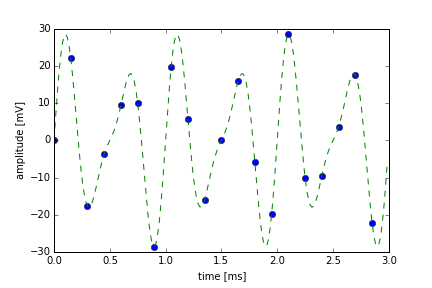
\includegraphics[width=0.55\textwidth]{figs/periodogram_ts.png}}\\
{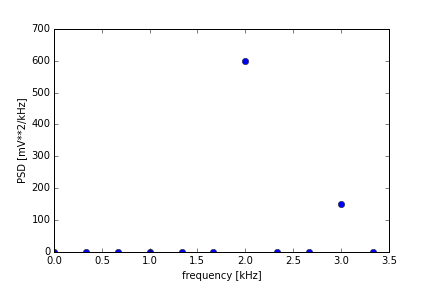
\includegraphics[width=0.55\textwidth]{figs/periodogram_eg.png}}
\end{center}
\caption{\label{fig:periodogram}  An example periodogram calculated from 20 samples over $3~\rm ms$ from a signal composed of two sine waves with amplitudes $10~\rm mV$ and $20~\rm mV$.  There are two peaks in the periodogram with PSD values $\mathcal{S}_{+}(f_n) = 150$ and $600~{\rm mV^2} / {\rm kHz}$ as expected from Equation~\ref{eqn:psdcalib}.
}
\end{figure}

\chapter{The Uncertainty Principle}
\section{The Fourier Transform in Quantum Mechanics}

So far we have been considering the Fourier transform with respect to position $x$ and wave-number $k$.  A much more useful pair of variables for Quantum Mechanics turns out to be momentum $p$ and position $x$.  To relate $p$ to $k$ we need only apply the DeBroglie relation to the wavelength in the definition of the wavenumber:
\begin{displaymath}
k \equiv \frac{2 \pi}{\lambda} = \frac{2 \pi p}{h} = \frac{p}{\hbar}
\end{displaymath}
We could therefore make the substitution $k \to p/\hbar$ (and $dk \to dp / \hbar)$) in Equations~\ref{eqn:ift} and ~\ref{eqn:ft}.  It turns out that a marginally more useful equation results if we make the normalization factors symmetric, by splitting the normalization factor of $1/\hbar$ across both equations with $1/\sqrt{\hbar}$ applied to each:
\begin{eqnarray} 
\Psi(x) &=& \frac{1}{\sqrt{2\pi\hbar}} \int_{-\infty}^{\infty} \widetilde{\Psi}(p) \exp(ipx/\hbar) \, dp \\
\widetilde{\Psi}(p) &=&  \frac{1}{\sqrt{2\pi\hbar}} \int_{-\infty}^{\infty} {\Psi}(x) \exp(-ipx/\hbar) \, dx
\end{eqnarray}
The major benefit of this symmetric form is that the normalization of $\Psi(x)$ and $\widetilde{\Psi}(p)$ in this case turns out to be the same:
\begin{displaymath}
\int_{-\infty}^{\infty} |\Psi(x)|^2 dx = \int_{-\infty}^{\infty} |\widetilde{\Psi}(p)|^2 dp = 1 
\end{displaymath}
Because we can always calculate $\Psi(x)$ from $\widetilde{\Psi}(p)$ either one completely describes the quantum mechanical state.  We call $\widetilde{\Psi}(p)$ the momentum wave function.   Whereas $|\Psi(x)|^2$ gives us the probability density for the quanton to be at position $x$, $|\Psi(p)|^2$ gives us the probability density for the quanton to have momentum $p$.

\section{The Uncertainty Principle}

Imagine that a particle is near $x=0$ with some uncertainty $\sigma_x$.  One way we might describe such a state is that the probability distribution is a Gaussian (bell-curve) distribution:
\begin{displaymath}
|\Psi(x)|^2 = N_x^2 \exp\left(-\frac{x^2}{2\sigma_x^2}\right)
\end{displaymath}
where $N_x$ is a normalization factor chosen such that 
\begin{displaymath}
\int_{-\infty}^{\infty} |\Psi(x)|^2 = 1.
\end{displaymath}
One wave function that would lead to such a probability distribution is 
\begin{displaymath}
\Psi(x) = N_x \exp\left(-\frac{x^2}{4\sigma_x^2}\right).
\end{displaymath}
Let's look at the momentum wave function for this particle:
\begin{eqnarray} 
\widetilde{\Psi}(p) &=&  \frac{1}{\sqrt{2\pi\hbar}} \int_{-\infty}^{\infty} {\Psi}(x) \exp(-ipx/\hbar) \, dx \\
&=&  \frac{N}{\sqrt{2\pi\hbar}} \int_{-\infty}^{\infty}  \exp \left(-\frac{x^2}{4\sigma_x^2} - \frac{ipx}{\hbar}\right) \, dx
\end{eqnarray}
The trick to solving this integral is called {\em completing the square}, we add and subtract the missing term needed to write this as $(x+a)^2 + b$:
\begin{eqnarray*} 
X &=&  -\frac{x^2}{4\sigma_x^2} - \frac{ipx}{\hbar} \\
&=&  -\frac{1}{4\sigma_x^2}(x^2 - 4ipx\sigma_x^2/\hbar) \\
&=&  -\frac{1}{4\sigma_x^2}(x^2 - 4ipx\sigma_x^2/\hbar  + 4i^2p^2\sigma_x^4/\hbar^2 - 4i^2p^2\sigma_x^2/\hbar^2) \\
&=&  -\frac{(x - 2 i p\sigma_x^2/\hbar)^2}{4\sigma_x^2} - p^2\sigma_x^2/\hbar^2
\end{eqnarray*}
The whole point of this is that because $x$ runs from $-\infty$ to $\infty$ we can now make a change of variables $x - 2 i p\sigma_x^2/\hbar \to x$ to clean things up dramatically:
\begin{eqnarray*} 
X &=&  -\frac{x^2}{4\sigma_x^2} - p^2\sigma_x^2/\hbar^2
\end{eqnarray*}
Our integral now becomes:
\begin{eqnarray} 
\widetilde{\Psi}(p) &=&  \frac{N}{\sqrt{2\pi\hbar}} \int_{-\infty}^{\infty}  \exp \left( -\frac{x^2}{4\sigma_x^2} - p^2\sigma_x^2/\hbar^2 \right) \, dx \nonumber \\
&=& \left\{ \frac{N}{\sqrt{2\pi\hbar}} \int_{-\infty}^{\infty}  \exp \left( -\frac{x^2}{4\sigma_x^2} \right) \right\} \exp\left( - p^2\sigma_x^2/\hbar^2 \right) \nonumber \\
&=& N_p \exp(-p^2 \sigma_x^2/\hbar^2) \label{eqn:psip}
\end{eqnarray}
Where in the last step we have noted that the term in brackets is just a constant and set $N_p=\{...\}$.

Fortunately the term in brackets ${}$ does not depend on $p$ at all... there's no need to calculate it, it will just give us a normalized momentum wave function.  We might it as well just set it to $N_p$:
Recall that we started with a wave function which had a Gaussian (bell-shaped) probability distribution with uncertainty $\sigma_x$:
\begin{displaymath}
|\Psi(x)|^2 = N_x^2 \exp\left(-\frac{x^2}{2\sigma_x^2}\right).
\end{displaymath}
We found that the momentum wave function also has a Gaussian probability distribution, if we call the uncertainty on the momentum $\sigma_p$, the probability distribution should have form the same form:
\begin{eqnarray*}
|\widetilde{\Psi}(p) |^2 &=& N_p^2 \exp\left(-\frac{p^2}{2 \sigma_p^2} \right)
\end{eqnarray*}
Comparing this to Equation~\ref{eqn:psip} we conclude:
\begin{displaymath}
\sigma_p = \frac{\hbar}{2 \sigma_x}
\end{displaymath}
or:
\begin{displaymath}
\sigma_x \sigma_p = \frac{\hbar}{2}
\end{displaymath}
Since uncertainties can always be worse than the best case, we have more generally:
\begin{displaymath}
\sigma_x \sigma_p \geq \frac{\hbar}{2}
\end{displaymath}
This is the Heisenberg uncertainty principle of quantum mechanics.  The more precisely the position is determined, the less precisely the momentum is determined, and vice versa.  It is a direct consequence of the wave like nature of matter.



\section{Exercises}

\noindent
{\bf Problem 1:} Show that the sines and cosines are orthogonal functions as claimed in Equations~\ref{eqn:trigortha}--\ref{eqn:trigorthc}.  You can compute the integrals using the trigonometric identities:
\begin{eqnarray*}
\sin \alpha \sin \beta &=& \frac{1}{2} \{\cos(\alpha - \beta) - \cos(\alpha + \beta)\}\\
\cos \alpha \cos \beta &=& \frac{1}{2} \{\cos(\alpha - \beta) + \cos(\alpha + \beta)\}\\
\cos \alpha \sin \beta &=& \frac{1}{2} \{\sin(\alpha + \beta) - \sin(\alpha - \beta)\}\\
\end{eqnarray*}
\vskip 0.5cm

\noindent
{\bf Problem 2:} There are different conventions for the constant term $C$ in Equation~\ref{eqn:bigseries}.
Since this is the only term that gives $f(x)$ a mean value, we must in every case have:
\begin{displaymath}
C = \frac{1}{L} \int_{-\frac{L}{2}}^{-\frac{L}{2}}  dx f(x).
\end{displaymath}
Show that we can extend Equation~\ref{eqn:coscos} so that
\begin{displaymath}
\braket{c_n,c_m} = \delta_{n m}
\end{displaymath}
even for $n=m=0$ for a suitable definition of the constant ``function" $c_0$.  Further show that then if we define $A_0 = \braket{c_0, f}$ then we must have $C = A_0/\sqrt{L}$.   A much more common approach is to extend Equations~\ref{eqn:convcoeffa} and \ref{eqn:convcoeffb} 
\begin{eqnarray*}
a_n  = \frac{2}{L} \int_{-\frac{L}{2}}^{\frac{L}{2}} 
f(x) \cos( k_n x) \, dx  \\
b_n  = \frac{2}{L} \int_{-\frac{L}{2}}^{\frac{L}{2}} 
f(x) \sin( k_n x) \, dx 
\end{eqnarray*}
to include $n=0$.  Show that in this case $b_0 = 0$ always, and that we must have $C = a_0/2$, just as in Equation~\ref{eqn:convseries}. \\
\vskip 0.5cm

\noindent
{\bf Problem 3:}  Consider the function $f(x) = x$ for the interval $[-1,1]$.  For its
Fourier Series representation following the convention of Equation~\ref{eqn:convseries}, calculate the coefficients $a_0$, $a_1$ and $b_1$.  What about $a_2$ and $a_3$? \\
\vskip 0.5 cm

\noindent
{\bf Problem 4:} Verify Equation~\ref{eqn:exportho} in two different ways: (a) by explicitly calculating the integral, and (b) by using Euler's Equation and the orthogonality of the sines and cosines.\\
\vskip 0.5cm

\noindent
{\bf Problem 5:} Using the compact form of the Fourier Series (Equation~\ref{eqn:complexseries}) show that the prescription for determining the coefficients (Equations~\ref{eqn:complexcoeff}) is valid.  Use the same method as was used at the end of Section~\ref{sect:coeff}. \\
\vskip 0.5cm


\noindent
{\bf Problem 6:} For the function $f(x) = \sin(2 \pi f_n x )$ find all of the non-zero Fourier coefficients in the Fourier Series of Equation~\ref{eqn:complexseries}.\\
\vskip 0.5cm

\noindent
{\bf Problem 7:}  Suppose that instead of being in an Eigenstate of Energy, a particle in a box has equal probability to be anywhere in the box, so the wave function is:
\begin{displaymath}
\Psi(x) = 
\left\{
	\begin{array}{ll}
		1/d  & \mbox{if } -d/2 < x < d/2 \\
		0 & \mbox{otherwise}
	\end{array}
\right.
\end{displaymath}
Compute the corresponding momentum wave function by taking the Fourier Transform.


\noindent
{\bf Problem 8:}  Short that the auto-correlation function $\mathcal{R}(\tau) = \braket{f(t)f^*(t-\tau)}$ of $f(t)=\exp(i2\pi f t)$ is simply $f(\tau)$.  Therefore, show that the PSD for $f(t)$ is a delta function at $f$.

\noindent
{\bf Problem 8:}  Short that the auto-correlation function $\mathcal{R}(\tau) = \braket{f(t)f^*(t-\tau)}$ of $f(t)=\exp(i2\pi f t)$ is simply $f(\tau)$.  Therefore, show that the PSD for $f(t)$ is a delta function at $f$.

\noindent
{\bf Problem 9:}  Suppose that a signal $f(t) = A \delta(t)$.  Calculate the autocorrelation function $R(\tau)=\int_{-\infty}^{+\infty} dt$ and then show that the Energy Spectral Density has the constant value $A^2$.

\appendix

\chapter{Informal Proofs}

A proper mathematical proof of these concepts requires about a one year course in mathematical analysis.  Fortunately, physicist are generally satisfied with informal proofs of mathematical concepts, because for us the ultimate validation of any hypothesis is experiment.

\section{The Dirac Delta Function}

These proofs make extensive use of the Dirac delta function, $\delta(x)$, which is zero everywhere but at $x=0$, where it is infinite.  Mathematically, the delta function only makes formal sense inside an integral, where it has the following defining properties:
\begin{eqnarray}
\int_{-\infty}^{\infty} f(x') \, \delta(x-x') \, dx' &=& f(x) \\
\int_{-\infty}^{\infty} \delta(x) \, dx &=& 1 \label{eqn:norm}
 \end{eqnarray}
The delta function simply picks out from the integral the one value of the integrand which makes the argument of the delta function non-zero.  The second equation shows the normalization of the delta function, which follows from the first if you take $f(x)=1$.

\section{The completeness of the sines and cosines}

\begin{figure}[thb]
\begin{center}
{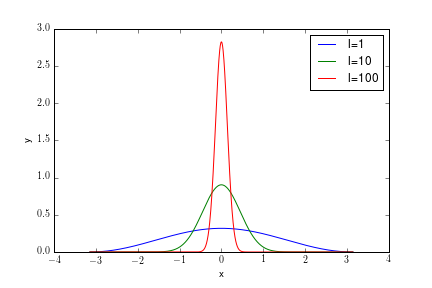
\includegraphics[width=0.40\textwidth]{figs/hk.png}}
\end{center}
\caption{\label{fig:hl} The function $h_\ell(x)$ for increasingly large values of $\ell$.}
\end{figure}

\noindent
To demonstrate the completeness of sines and cosines\footnote{This proof taken from http://web.mit.edu/jorloff/www/18.03-esg/notes/fourier-complete.pdf} we construct a peculiar but useful set of functions defined for $\ell=1,2,3,...$:
\begin{displaymath}
h_\ell(x) = c_\ell \left(\frac{1 + \cos(x)}{2}\right)^\ell
\end{displaymath}
We chose each factor $c_\ell$ such that:
\begin{displaymath}
\int_{-\pi}^{\pi} h_\ell(x) = 1
\end{displaymath}
The shape of $h_\ell$ is shown in Fig.~\ref{fig:hl}.  As $\ell$ increases, $h_\ell$ becomes more and more narrow at $x=0$, while the normalization is as in Equation~\ref{eqn:norm}.  It looks more and more like the delta function:
\begin{displaymath}
\lim_{\ell \to \infty} h_\ell(x) = \delta(x)
\end{displaymath}
It has one other important feature:  $h_\ell(x)$ is simply a sum of cosines of $nx$ with coefficients that don't depend on $x$.  To see how this can be, note that we can always turn a product of cosines into a sum via the trigonometric identity:
\begin{displaymath}
\cos \alpha \cos \beta = \frac{1}{2} \{\cos(\alpha - \beta) + \cos(\alpha + \beta)\}.
\end{displaymath}
So, for instance, we can write:
\begin{eqnarray*}
h_2(x) &=& \frac{c_2}{4} + \frac{c_2\cos(x)}{2}+\frac{c_2\cos^2(x)}{4} \\
           &=& \frac{c_2}{4} + \frac{c_2\cos(x)}{2}+\frac{c_2\cos(2x)}{8}
\end{eqnarray*}
This property implies that the function $h_\ell(x-a)$ for some constant $a$ is simply a sum of {\em both} sines and cosines of $nx$ with coefficients that don't depend on $x$, as:
\begin{displaymath}
\cos(nx-na) = \cos(nx)\cos(na) + \sin(nx)\sin(na).
\end{displaymath}

With this technology in hand we are ready to demonstrate the completeness of the sines and cosines.   
For simplicity, it suffices to consider only functions with period $L=2\pi$ (i.e. $k_n=n$).  The general case can then be inferred by transformation of coordinates.  Consider a real function $f(x)$ which is periodic for $L=2\pi$.  For now just define the function $F(x)$ to be the infinite series:
\begin{eqnarray}
F(x) \equiv a_0 + \sum_{n=1}^{\infty}  \left\{ a_n \, \cos(n x ) + b_n \, \sin(n x ) \right\}.
\end{eqnarray}
This is the compact form of the Fourier Series for this special case $L=2\pi$, so $k_n = n$.
We assume the coefficients are determined in the usual way:
\begin{eqnarray*}
a_n &=& \frac{2}{L} \int_{-\frac{L}{2}}^{\frac{L}{2}} 
f(x) \cos(n x) \, dx  \\
b_n &=& \frac{2}{L} \int_{-\frac{L}{2}}^{\frac{L}{2}} 
f(x) \sin(n x) \, dx.
\end{eqnarray*}
We need to show that $F(x) = f(x)$, or 
\begin{displaymath}
g(x) = F(x) - f(x) = 0
\end{displaymath}
The proof hinges on the fact that $F(x)$ and $f(x)$ have the same Fourier coefficients, so that:
\begin{eqnarray*}
\int_{-\pi}^{\pi} g(x) \sin(nx) dx &=& \int_{-\pi}^{\pi} F(x) \sin(nx) dx -  \int_{-\pi}^{\pi} f(x) \sin(nx) dx \\
&=& b_n - b_n \\
&=& 0 \\
\int_{-\pi}^{\pi} g(x) \cos(nx) dx &=& \int_{-\pi}^{\pi} F(x) \cos(nx) dx -  \int_{-\pi}^{\pi} f(x) \cos(nx) dx \\
&=& a_n - a_n \\
&=& 0 
\end{eqnarray*}
This shows that the integral of $g(x)$ times any sine or cosine is zero.  But our special function $h_\ell(x-a)$ function is just a sum of sines and cosines of $nx$ for any value of $a$.  This means that:
\begin{eqnarray*}
\int_{-\pi}^{\pi} h_\ell(x-a) g(x) dx &=& 0 \\
\end{eqnarray*}
If we take the limit as $\ell \to \infty$, we obtain:
\begin{eqnarray*}
\int_{-\pi}^{\pi} \delta(x-a) g(x) dx &=& 0 \\
g(a) &=& 0 \\
\end{eqnarray*}
Since this is true for any value of $a$, we have $g(x) = 0$ and so $F(x) = f(x)$.

\section{The orthogonality and completeness of the complex exponential function}

The first thing we need to show is that:
\begin{equation}
\frac{1}{2\pi} \int_{-\infty}^{\infty} \exp(ikx) \, dk = \delta(x)
\end{equation}
To see this we first calculate:
\begin{eqnarray*} 
\frac{1}{2\pi} \int_{-a}^{a} \exp(ikx) \, dk &=& \frac{1}{2\pi} \, \frac{\exp(iax)-\exp(-iax)}{ix}\\
&=& \frac{1}{\pi} \, \frac{\sin(ax)}{x} \\
&=& \frac{a}{\pi} \, {\rm sinc}(ax)
\end{eqnarray*}
An integration shows that:
\begin{eqnarray}
\int_{-\infty}^{\infty} \frac{a}{\pi} \, {\rm sinc}(ax) \, dx = 1
\end{eqnarray}
exactly as needed for Equation~\ref{eqn:norm}.

Fig.~\ref{fig:sinc} shows that this function peaks at zero and becomes more and more narrow for progressively larger values of $a$.  Since it has the correct normalization, we conclude that:
\begin{eqnarray}
\frac{1}{2\pi} \int_{-\infty}^{\infty} \exp(ikx) \, dk &=& \lim_{a\to\infty} \frac{1}{2\pi} \int_{-a}^{a} \exp(ikx) \, dk \nonumber \\
&=& \lim_{a\to\infty} \frac{a}{\pi} \, {\rm sinc}(ax) \nonumber \\ 
&=& \delta(x) \label{eqn:delta}
\end{eqnarray}

\begin{figure}[thb]
\begin{center}
{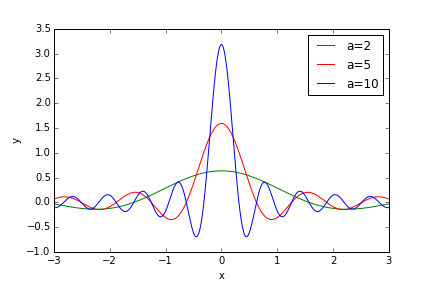
\includegraphics[width=0.40\textwidth]{figs/sinc.png}}
\end{center}
\caption{\label{fig:sinc} The function $a \, {\rm sinc}(ax)/\pi$ for progressively larger values of $a$.  As $a \to \infty$, this function approaches the delta function $\delta(x)$.}
\end{figure}

We are now fully equip to show that the complex exponential functions:
\begin{equation*}
e_k = \frac{1}{\sqrt{2\pi}} \exp(i k x)
\end{equation*}
are orthonormal.  Calculating the inner product
\begin{eqnarray*}
\braket{e_k, e_{k'}} &=& \int_{-\infty}^{\infty} \frac{1}{\sqrt{2 \pi}}  \exp(-ikx) \frac{1}{\sqrt{2 \pi}}  \exp(ik'x) \, dx \\
                               &=& \frac{1}{2 \pi} \int_{-\infty}^{\infty} \exp\{i(k'-k)x\} \, dx \\
                               &=& \delta(k-k')
\end{eqnarray*}
where we have used Equation~\ref{eqn:delta} but with the roles of $x$ and $k$ exchanged.
To prove completeness, we can now show that:
\begin{eqnarray*}
\Psi(x) &=& \int_{-\infty}^{\infty} \Psi(x') \, \delta(x-x') \, dx' \\
&=& \int_{-\infty}^{\infty} f(x') \left\{ \frac{1}{2 \pi} \int_{-\infty}^{+\infty} \exp\{ik(x-x')\} \, dk \right\} \, dx' \\
&=& \frac{1}{\sqrt{2 \pi}} \int_{-\infty}^{\infty} \left\{ \frac{1}{\sqrt{2 \pi}} \int_{-\infty}^{+\infty} f(x') \exp(-ikx') \, dx' \right\}  \exp(ikx) \, dk \\
&=& \frac{1}{\sqrt{2 \pi}} \int_{-\infty}^{\infty} \widetilde{\Psi}(k)  \exp(ikx) \, dk \\
\end{eqnarray*}
where:
\begin{eqnarray*}
\widetilde{\Psi}(k) &=& \frac{1}{\sqrt{2\pi}} \int_{-\infty}^{\infty} \Psi(x) \, \exp(-ikx) \, dx \\
\end{eqnarray*}

\section{The Nyquist--Shannon sampling theorem}

Consider a continuous function $V(t)$ with Fourier transform $\widetilde{V}(f)$ that does not contain any frequencies larger than $B$, i.e. $\widetilde{V}(f) = 0$  when $f>B$ or $f<-B$.  For simplicity, we'll assume that $\widetilde{V}(B) = \widetilde{V}(-B) = 0$.

Now consider the function $U(x)$ defined by:
\begin{displaymath}
U(x) \equiv \sum_{m=-\infty}^{\infty} \widetilde{V}(m2B-x)
\end{displaymath}
which has been constructed to be a periodic function of $x$, with period $2B$.
If we can obtain $U(x)$, then we can also easily obtain $\widetilde{V}(f)$, because $\widetilde{V}(f) = U(-f)$ in range $-B \leq f \leq B$ and is zero elsewhere.

$U(x)$ is periodic with period $2B$, and so it has a Fourier Series representation:
\begin{displaymath}
U(x) = \sum_{n=-\infty}^{\infty} c_n \exp(i k_n f) 
\end{displaymath}
where $k_n = 2 \pi n / 2B$.   We can obtain the coefficients as follows:
\begin{eqnarray*}
c_n &=& \frac{1}{2B} \int_{-B}^{B} dx \; U(x) \, \exp(i 2 \pi n x / 2B)\\
&=& \frac{1}{2B}  \sum_{m=-\infty}^{\infty} \int_{-B}^{B} dx \; \widetilde{V}(m2B-x) \, \exp(i 2 \pi n x / 2B)
\end{eqnarray*}
But $-B \leq x \leq B$, so $\widetilde{V}(m2B-x) = 0$ whenever $m \neq 0$, and so:
\begin{eqnarray*}
c_n &=& \frac{1}{2B} \int_{-B}^{B} dx \; \widetilde{V}(-x) \, \exp(i 2 \pi n x / 2B) \\
&=& \frac{1}{2B} \int_{-B}^{B} df \; \widetilde{V}(f) \, \exp(-i 2 \pi n f / 2B) \\
&=& \frac{V(n / 2B)}{2B}
\end{eqnarray*}
That is, the discrete coefficients $c_n$ can be determined from the continuous function $V(t)$ sampled at the discrete times $t = n / 2B$.  From the coefficients $c_n$ we obtain the function $U(x)$, and so $\widetilde{V}(f)$, and from the Fourier transform $\widetilde{V}(f)$ we can of course determine the function $V(t)$.  Therefore, the complete continuous function $V(t)$ can be calculated from it's values sampled at the discrete times $t = n / 2B$. 




\end{document}




